%-------------------------------------------------------------------------
% Design Project Input/Output Module Description
%-------------------------------------------------------------------------

\clearpage
\section{Infrared (IR) Input Module}
\label{sec-input-ir}

This input module enables your IoT device to sense the distance to an
object placed \wu{10--80}{cm} in front of it, using the same Sharp
GP2Y0A21 Distance Sensor you possibly experimented with in Lab~2. The
sensor works by bouncing infrared (IR) light off objects and sensing the
angle at which it returns; a process called \IT{triangulation}. The
figure below to the left shows IR light bounced off an object placed at
two different distances -- notice how knowing the angle of reflected
light tells you the object's distance. The output of the sensor is a
voltage, corresponding to the distance derived from the angle of
reflected light. Moving an object to different distances changes the
output voltage as shown in the figure below to the right. Can you see
why the range of this device is chosen to be \wu{10--80}{cm}?

\vspace{0.1in}
\begin{minipage}[t]{0.49\tw}
  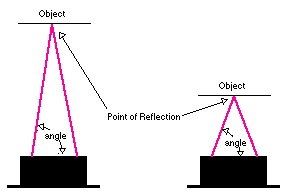
\includegraphics[width=\tw]{ir-sensor-triangulation.jpg}
\end{minipage}
\hfill
\begin{minipage}[t]{0.49\tw}
  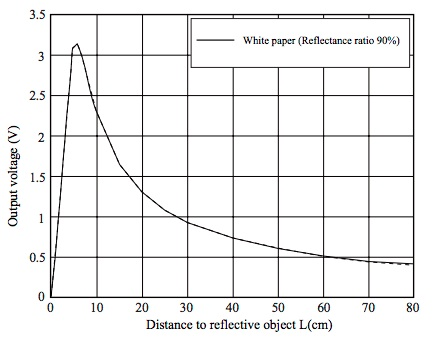
\includegraphics[width=\tw]{ir-sensor-response-curve.jpg}
\end{minipage}
\vspace{0.1in}

A sample circuit and Arduino code is shown below to get you started.
There is no need for any extra components; we directly connect the blue
wire from the IR sensor to an analog input on the Arduino. The example
code will print the analog reading from the IR sensor on the serial
monitor, similar to how we printed the analog reading from the grayscale
sensor in Lab~2. After setting up the circuit and programming the
Arduino, open the serial monitor and experiment with placing objects
(e.g., a book) at various distances away from the front of the sensor.
The reading from the sensor should be larger for objects farther away
from the sensor and smaller for objects closer to the sensor.

\vspace{0.1in}
\begin{minipage}[t]{0.49\tw}
  \vspace{0pt}

  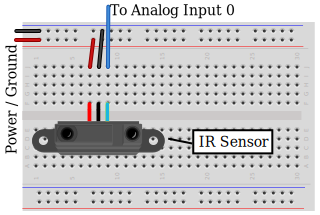
\includegraphics[width=\tw]{input-ir-annotated.svg.pdf}
\end{minipage}
\hfill
\begin{minipage}[t]{0.49\tw}
  \vspace{0.1in}
  \begin{Verbatim}[gobble=3,fontsize=\small]
    int pin_ir = A0;

    void setup() {
      Serial.begin(9600);
      pinMode( pin_ir, INPUT );
    }

    void loop() {
      int distance = analogRead( pin_ir );
      Serial.println( distance );
      delay(1000);
    }
  \end{Verbatim}
\end{minipage}
\vspace{0.1in}

Questions: (1) What happens if the object is further than 80cm (max
range) from the sensor? (2) What happens if the object is closer than
10cm (min range) from the sensor? (3) The sensor is not outputting
distance in any particular unit. How can we convert the readings into
centimeters?

